
        \begin{figure}[!t]
            \centering
            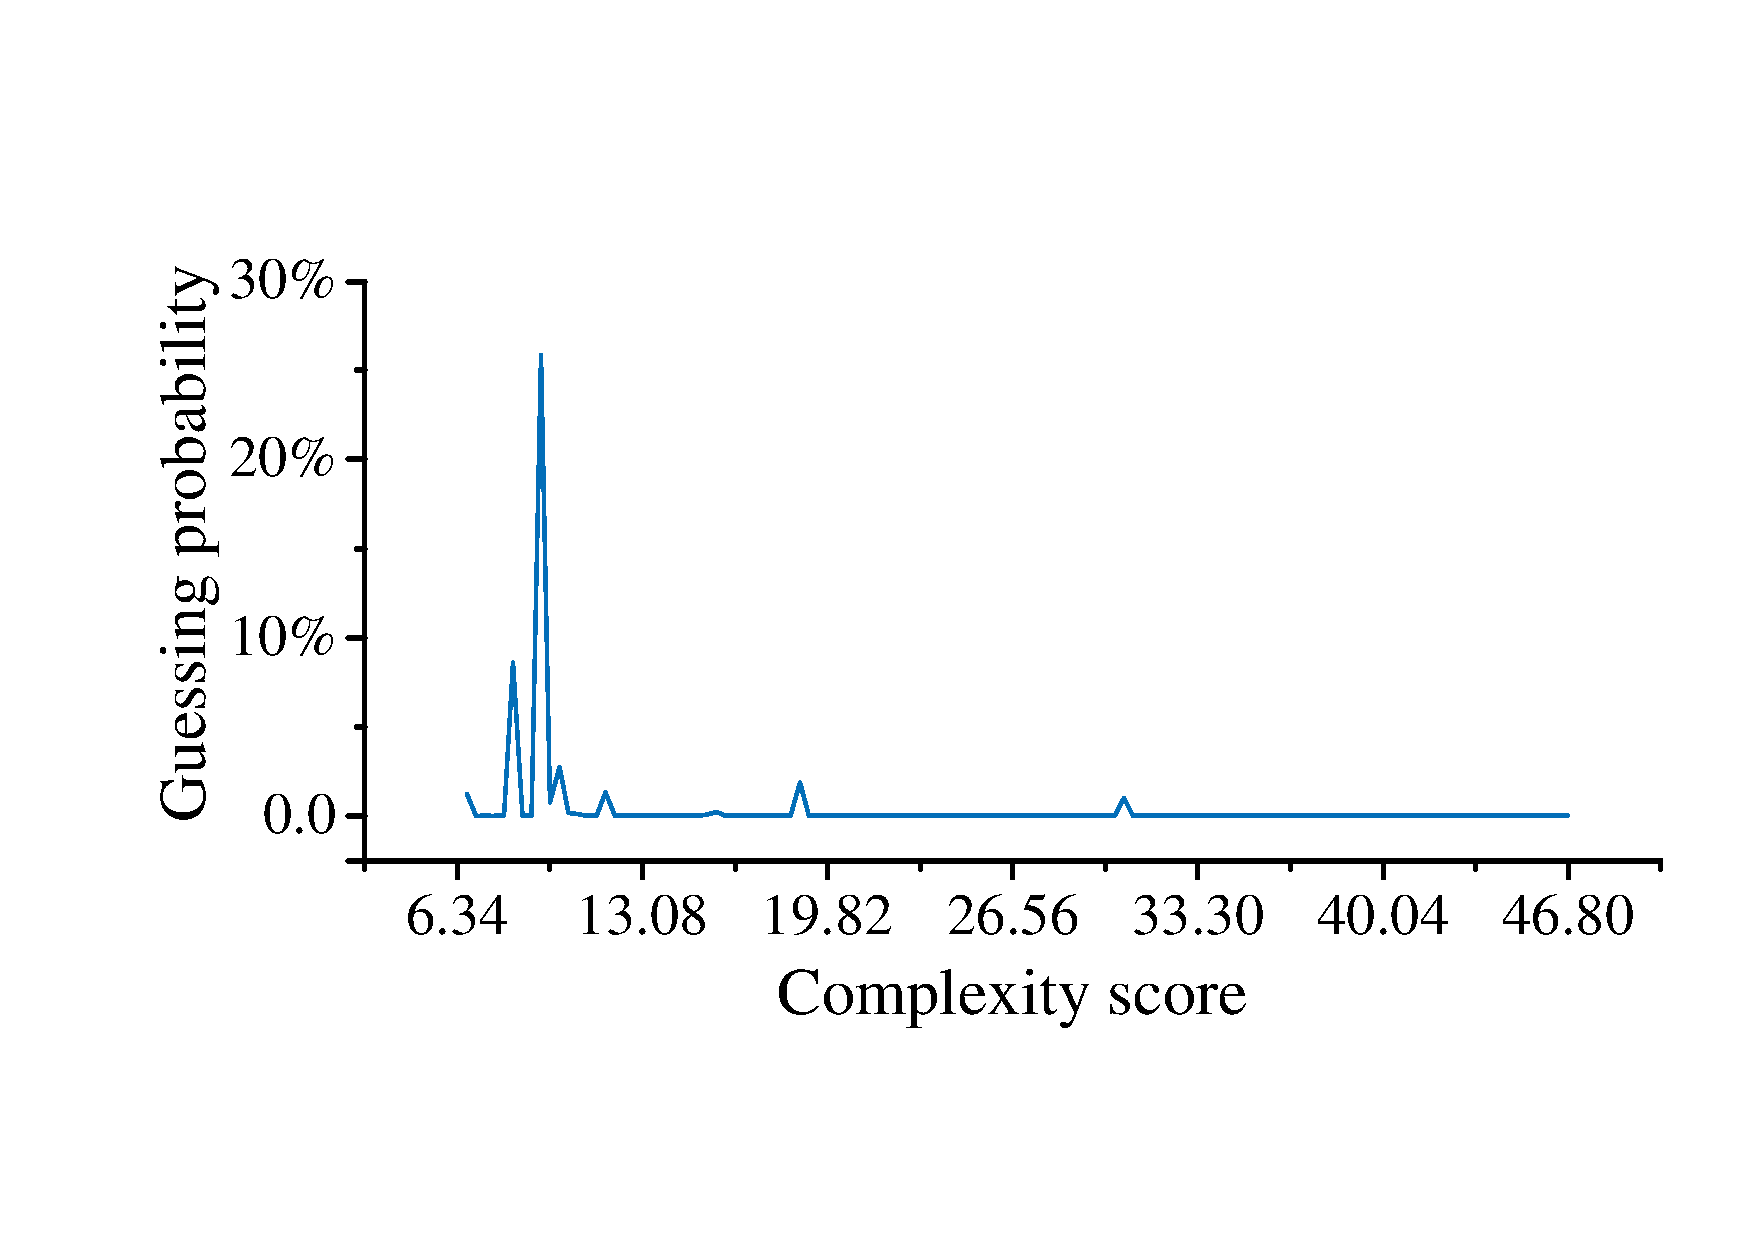
\includegraphics[width=0.5\textwidth]{fig/guess_prob.pdf}
            \caption{How likely a pattern can be guessed in five attempts as the complexity score increases. Patterns with a complexity score that is greater than 13 are
             unlikely to be guessed by an attacker within five attempts.}
            \label{fig:guessing-probability}
        \end{figure}

\section{Experimental Setup \label{sec:setup}}
    \subsection{Data Collection}
    \label{section:locking patterns}
    The patterns used in our evaluation were collected from users who use at least one Android device (a smartphone or a tablet) on a daily basis.
    To collect the patterns, we have distributed over 1,000 survey forms and collected back 215 valid forms, resulting in 120 unique patterns\footnote{Available to be downloaded from: \url{https://dx.doi.org/10.17635/lancaster/researchdata/113}}.
    Our participants include 95 females and 120 males who were undergraduate or postgraduate students in our institution.
    The majority of our participants are in an age group of under 30.

    To collect the patterns, we have conducted a ``pen-and-paper" survey by asking participants to fill in an anonymized questionnaire.
    The questionnaire and survey were approved by the research ethics board (REB) of the host institution.
    We have made sure that our survey complied with strict privacy regulations. For example, we did not collect any personally identifiable information other than the gender and age group of the participant. Our participants were well informed on the purpose
    of the study and how the data will be managed and used. The survey forms were distributed as voluntary homework so that the participants can take the survey form away to fill in.
     Users were invited to return the survey form anonymously within three weeks to a dedicated, locked mailbox, if they wish to participate in the study.
     To avoid a user submits multiple copies of the same form, each survey form is given a unique, randomly generated 32-digital number.
     %The list of patterns we collected and the questionnaire can be found in the Appendix.


     Overall, 37.6\% of our participants confirmed that they use pattern lock as the screen lock to
     protect their Android devices on a daily basis; and 33\% of those  who do not use a pattern as their screen lock said that they
     are often required to use a pattern for authentication by an application like \texttt{Alipay}. Furthermore, 60\%
     of our participants also indicated that the pattern they provided is currently being used
     or have been used in the past by themselves. Other participants (often those did not use a locking pattern on a daily basis) indicated that they
     have provided a pattern which they would like to use if a locking
     pattern is required. Based on this information, we are confident
     that the patterns we collected represent some of the real world
     patterns. Finally, all participants believe that a complex pattern provides stronger protection than a simple counterpart.

    \subsection{Pattern Complexity Classification}
    \label{section: pattern-complexity-classification}
    We quantify the complexity of a pattern using the complexity (strength) score proposed in~\cite{sun2014dissecting}.
        The complexity score, $CS_{P}$, of a pattern, $P$, is defined as:
    \begin{equation}
      CS_{P}=S_{P}\times\log_{2}(L_{P}+I_{P}+O_{P})
    \label{equ:compscore}
    \end{equation}
    where $S_{P}$ is the number of connected dots, $L_{P}$ is the
    total length of all line segments that form the pattern (see
    Figure~\ref{fig:intersection-overlap}~a), $I_{P}$ is the number of
    intersections (which are also termed as "knight moves" in some prior
    work~\cite{Von2015Easy}, see
    Figure~\ref{fig:intersection-overlap}~b) and $O_{P}$ is the number of
    overlapping linear segments (see
    Figure~\ref{fig:intersection-overlap}~c).  To calculate the line length,
    we assume the length between two horizontally or vertically adjunct dots
    is one. Thus, our method is independent of the size of the screen and the
    grid.


    Intuitively, the more connected dots ($S_{P}$), line segments ($L_{P}$),
    intersections ($I_{P}$) and overlapping line segments ($O_{P}$) that a
    pattern has, the more complex it is. For example, the patterns shown in
    Figure~\ref{fig:fig8} (c) use all the nine dots of the grid, and have  at
    least seven line segments and three intersections.
    There are other methods to quantify the complexity score of pattern locks, including the methods proposed by Song \emph{et al.} ~\cite{Song2015On} and Andriotis \emph{et al.}
    ~\cite{Andriotis2014Complexity}. These methods in general suggest that patterns with more connected dots and intersections are considered to provide stronger security strengths~\cite{Heidt2016Refining}.

        \begin{figure}[!t]
            \centering
            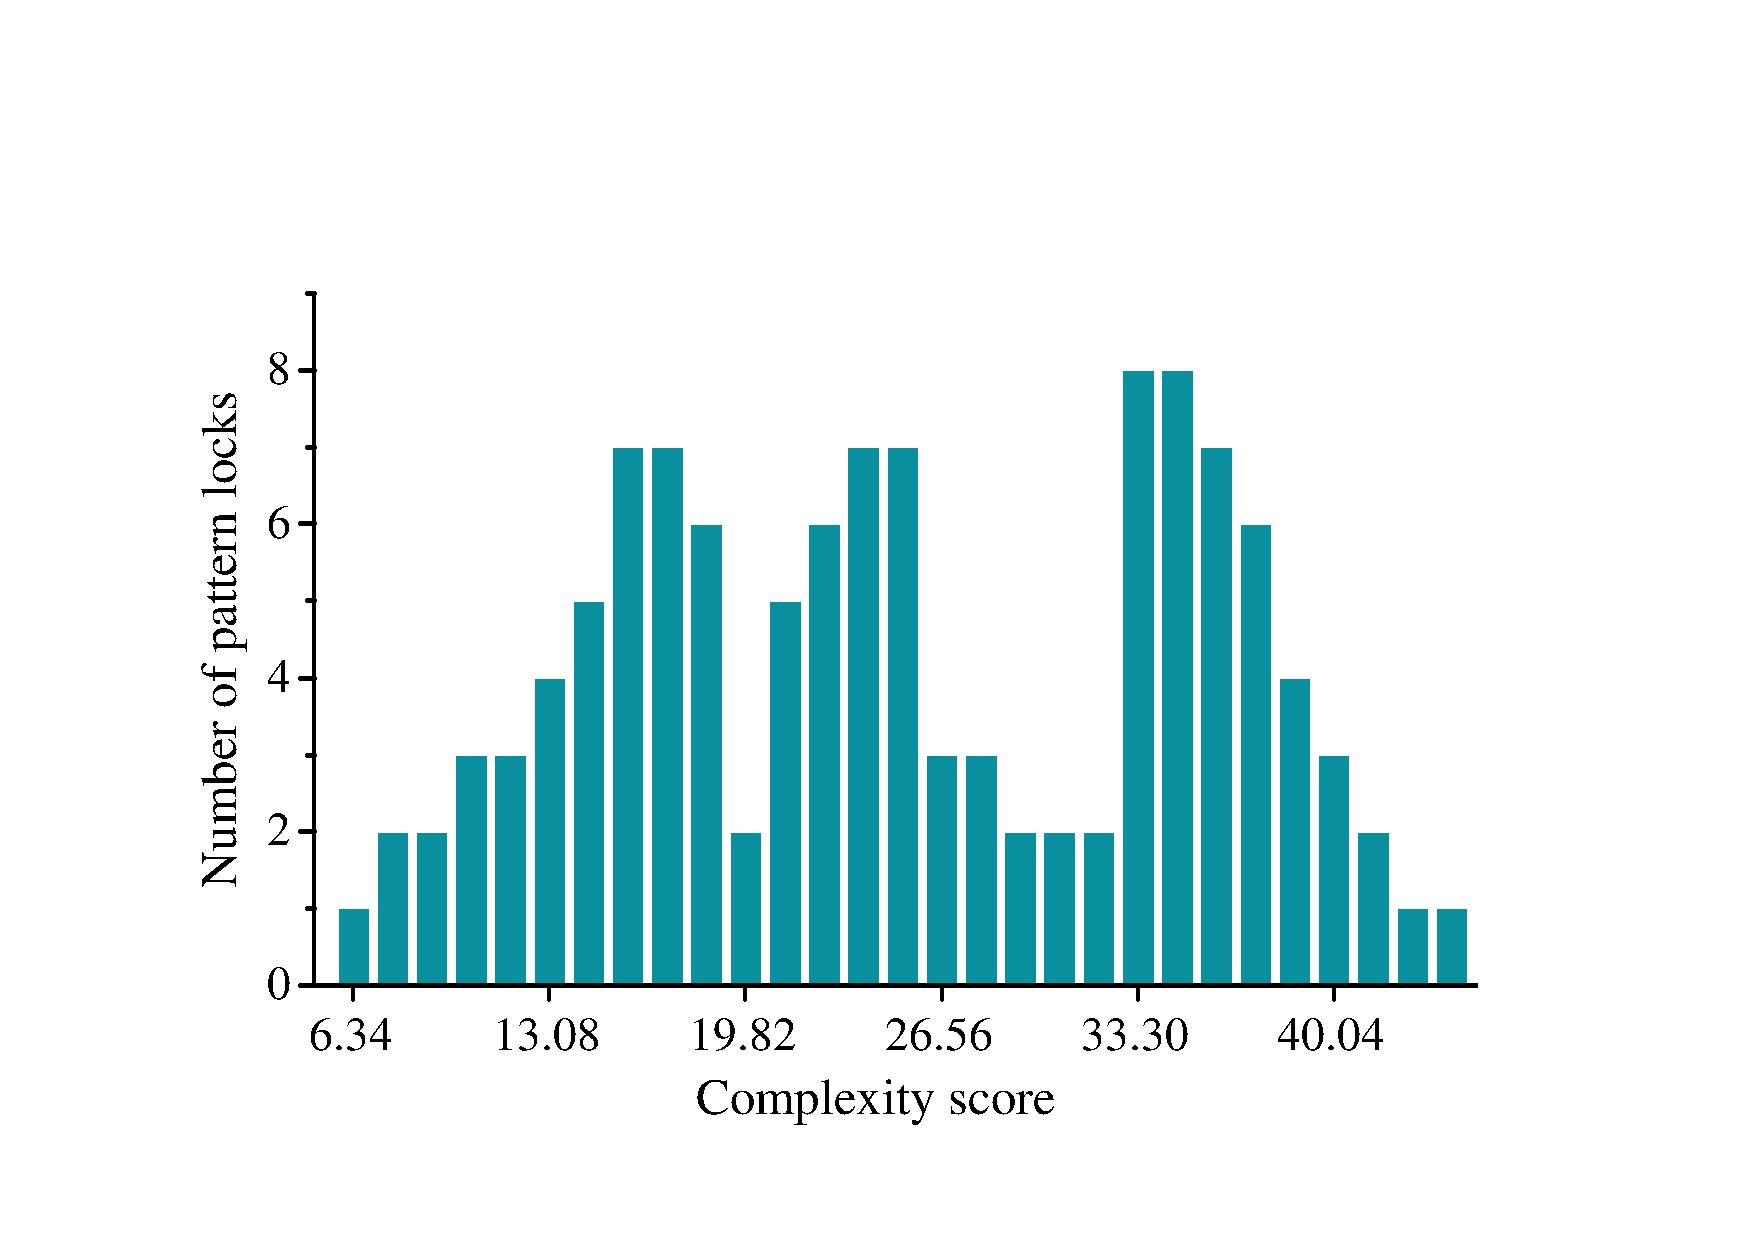
\includegraphics[width=0.5\textwidth]{fig/pattern-strength.pdf}
            \caption{The distribution of complexity scores for the patterns given by our participants.}
            \label{fig:pattern-strength}
        \end{figure}

    \begin{table}[!t]
            \centering
            \caption{Screen sizes for the test phones}
            \label{tab:locking-screen-size}
            \small
            \begin{tabular}{cccc}
                %\includegraphics[width=7.5cm]{fig/table1.pdf}
                \toprule
                \textbf{Screen size} & \textbf{MI4} & \textbf{Honor7} & \textbf{Note4} \\
                \midrule
                Height(cm)$\times$Width(cm) & $13.9\times6.9$ & $14.3\times7.2$ & $15.4\times7.9$ \\
                \bottomrule
            \end{tabular}
            %\vspace{-4mm}
    \end{table}

    Figure~\ref{fig:guessing-probability} illustrates how the guessing probability\footnote{A guessing probability is
    how likely an attacker can successfully guess a given pattern within five attempts.} changes as the complexity score (given by Equation~\ref{equ:compscore}) of the pattern lock changes.
    The probability is calculated on the set of patterns collected from our participants, by using the pattern strength
    measurement method proposed in \cite{Heidt2016Refining}. As can be seen from this diagram,
    our complexity score is inline with classical approaches for quantifying the security strength of pattern lock -- the more complexity a
    pattern is, the less likely it can be successfully guessed within 5 attempts.

    %\FIXME{explain the diagram – e.g. what are primitive curve and logistic fit!}.
   % \FIXED{the primitive curve presents the relevance between the guessing probability and the complexity scores. It directly reveals how likely a pattern can be guessed within five attempts as the complexity score increases. The trend of the primitive curve is shown by the logistic fit curve (the red dash curve), which indicates that a pattern with higher complexity score (typically more than 13) is hard to be guessed within five attempts.}

    \vspace{2mm}
    \noindent \textbf{Pattern Grouping.}
    Base on the complexity score, we divide the collected patterns into three complexity categories: \emph{simple}, \emph{median} and \emph{complex}. A simple pattern has a score of less than 19,
    a median
    complex pattern has a score between 19 and 33, and a complex pattern must have a score greater than 33. This classification gives us roughly 40 patterns per
    category. Figure~\ref{fig:fig8} gives some examples for each category while Figure~\ref{fig:pattern-strength} shows the distribution of these patterns according to their complexity scores.
    Based on this definition, the most complex pattern on a $3 \times 3$ grid has a score of $46.8$ (see Figure~\ref{fig:most complex patterns}).  The complex scores of the patterns we collected range from $6.4$ to $46.8$.

        \begin{figure}[!t]
            \centering
            \subfigure{
                \begin{minipage}[b]{0.12\textwidth}
                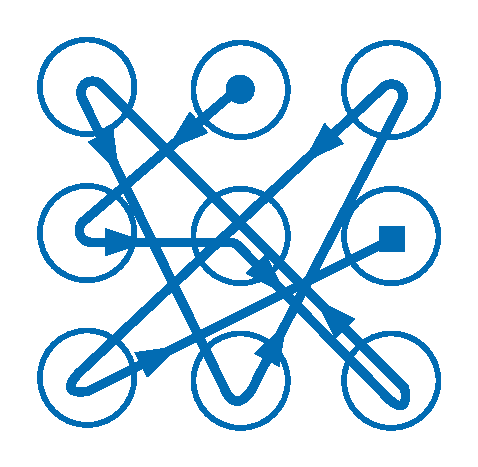
\includegraphics[width=\textwidth]{fig/complex3.pdf} \\
                \centering  complexity score: $43.8$
                \end{minipage}
            }
            \subfigure{
                \begin{minipage}[b]{0.12\textwidth}
                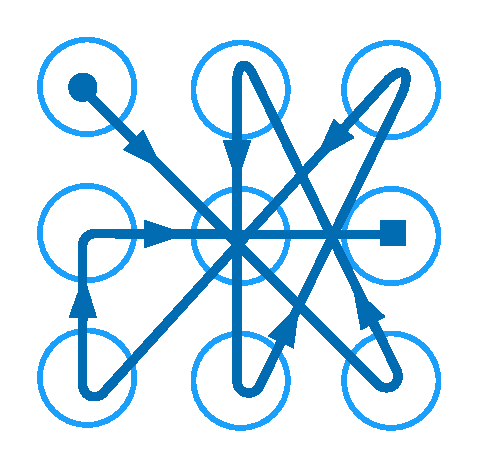
\includegraphics[width=\textwidth]{fig/complex2.pdf} \\
                \centering  complexity score: $44.7$
                \end{minipage}
            }
            \subfigure{
                \begin{minipage}[b]{0.12\textwidth}
                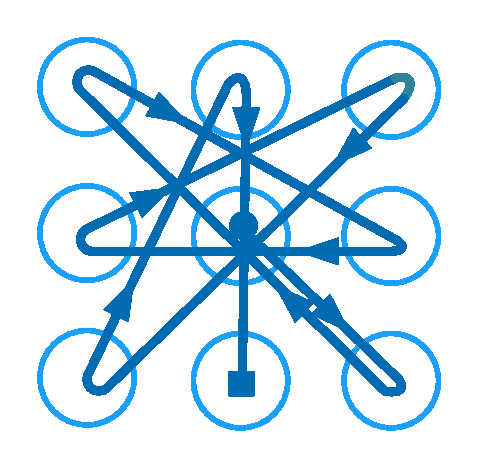
\includegraphics[width=\textwidth]{fig/complex1.pdf} \\
                \centering  complexity score: $46.8$
                \end{minipage}
            }
            \vspace{-2mm}
            \caption{Three most complex patterns on a $3\times 3$ grid based on Equation~\ref{equ:compscore}.}
            \vspace{-2mm}
            \label{fig:most complex patterns}
        \end{figure}

    \subsection{Video Recording and Preprocessing}

    \noindent\textbf{User Participation} We recruited ten postgraduate students (five male and five female
    students) from Northwest University to reproduce the 120 patterns (collected from users)
    and the 60 most complex patterns (see Section~\ref{sec:overall_rate})  on three target mobile phones:
    a Xiaomi MI4, a Huawei Honor7 and a Samsung Note4. Table~\ref{tab:locking-screen-size} lists
    the screen size for each target mobile phone.

    \vspace{2mm}
    \noindent\textbf{Recording Devices} We used three smartphones for video recording: an Apple iPhone4S,
     a Xiaomi MI4 and a Meizu2. Each mobile phone was used to record 40 patterns with a
    1080p HD resolution of 30 FPS under different settings described as follows.

    \vspace{2mm}
   \noindent\textbf{Video Recording Setup.}
    By default, we used the  Android $3 \times 3$ native pattern grid,
    but we evaluated our approach using other pattern grids with different sizes in
    Section~\ref{sec:scalability}. We recorded each pattern under three filming
    angles, 45, 90 and 135 degrees, by placing the camera on the left-front, front, and right-front
    of the target device respectively.
    By default, the video
    was recorded indoor during daytime under a natural lighting condition. In
    Section~\ref{sec:light} we evaluated our approach under different lighting conditions
    both indoor and outdoor. By default, videos were recorded at a distance of
    2 meters from the target device and we evaluated the impact of the filming distance in
    Section~\ref{sec:scalability}.

    \vspace{2mm}
    \noindent \textbf{Video Filming.}
     Before recording, our participants were given the opportunity to practice a pattern
    several times, so that they can draw the pattern at
    their natural speed. On average, this practice session took 10 trails per user per pattern.
    When drawing the
    pattern, some participants sat, while others stood, some hold the device
    by hands, while others placed it on a table.
    Each pattern was drawn on three target devices and
    recorded under three filming angles. Thus, for the 120 patterns collected from users, we recorded 1,080 videos in total.

    \vspace{2mm}
    \noindent\textbf{Video Preprocessing.}
    For each video stream, we used the algorithm described in Section~\ref{sec:identify} to cut out the video segment
    of the unlocking process. We left around 200 to 300 milliseconds of the video segment before and after the pattern unlocking process.
    To track the fingertip locations,
    we used Windows Movie Make to highlight two areas of interest on the first frame of
    the video segment: one area surrounds the fingertip, and the other contains an edge of the
    phone (see Section~\ref {secction:shake}).

    \vspace{2mm}
   \noindent\textbf{Implementation.} Our prototyped attacking system built upon a TLD library~\cite{TLD-toolbox-web}.
    The developed software ran on an Intel Core i5 PC with
    8GB RAM. The operating system is Windows 10. Our implementation can be ported onto
    Android or Apple iOS systems, which is our future work. On our evaluation
    platform, our software takes less than 30 seconds to process a video to produce candidate patterns.
